\chapter{Methods}
\begin{itemize}
\item Introduce requirements
\item Need to preserve spatial information for symbolic front-end
\item Need disentangled latent space for symbolic front-end
\item Explain degree of freedom here (disentangled filters, or disentangled neurons, or something else?)
\item This is unexplored territory here - we decide what the reasonable architecture should be
\end{itemize}

\label{ch:methods}


%
%
%
%
%
\section{Single Latent Filter}

\begin{itemize}
\item As mentioned, the type and position of an object must be preserved in the latent space
\item This may be achieved by using a single latent filter, with the object type corresponding to the value of the weighted sum of the neuron.
\end{itemize}

\subsection{Architecture}
\begin{figure}[H]
\centering
\captionsetup{justification=centering}
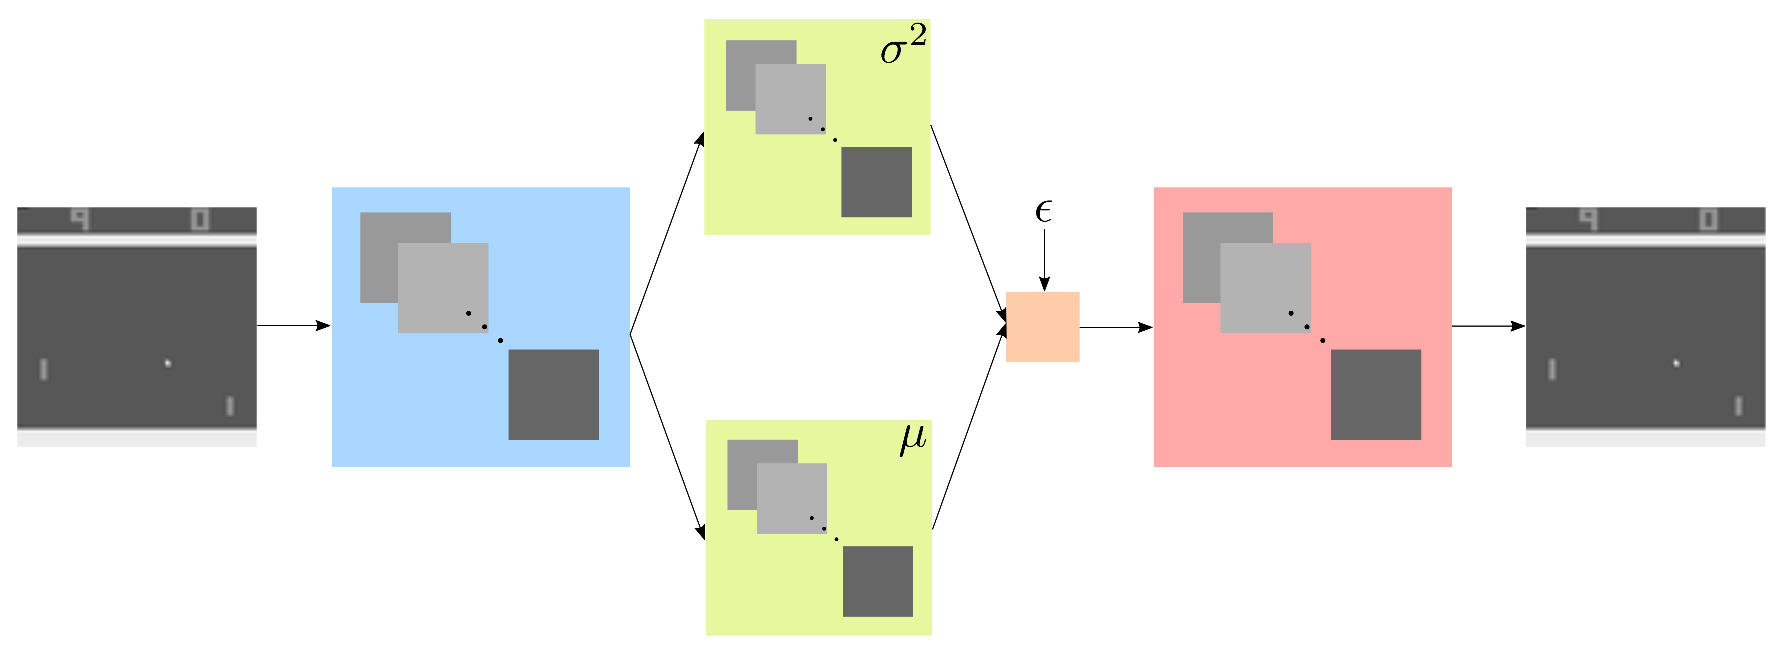
\includegraphics[scale=0.58]{methods/latent_image_architecture.eps}
\caption{Caption.}
\label{fig:latent_image_architecture}
\end{figure}

\subsection{Derivation}

%
%
%
%
%
\section{Disentangling Latent Neurons}
\lipsum[2]
\subsection{Architecture}
\begin{figure}[H]
\centering
\captionsetup{justification=centering}
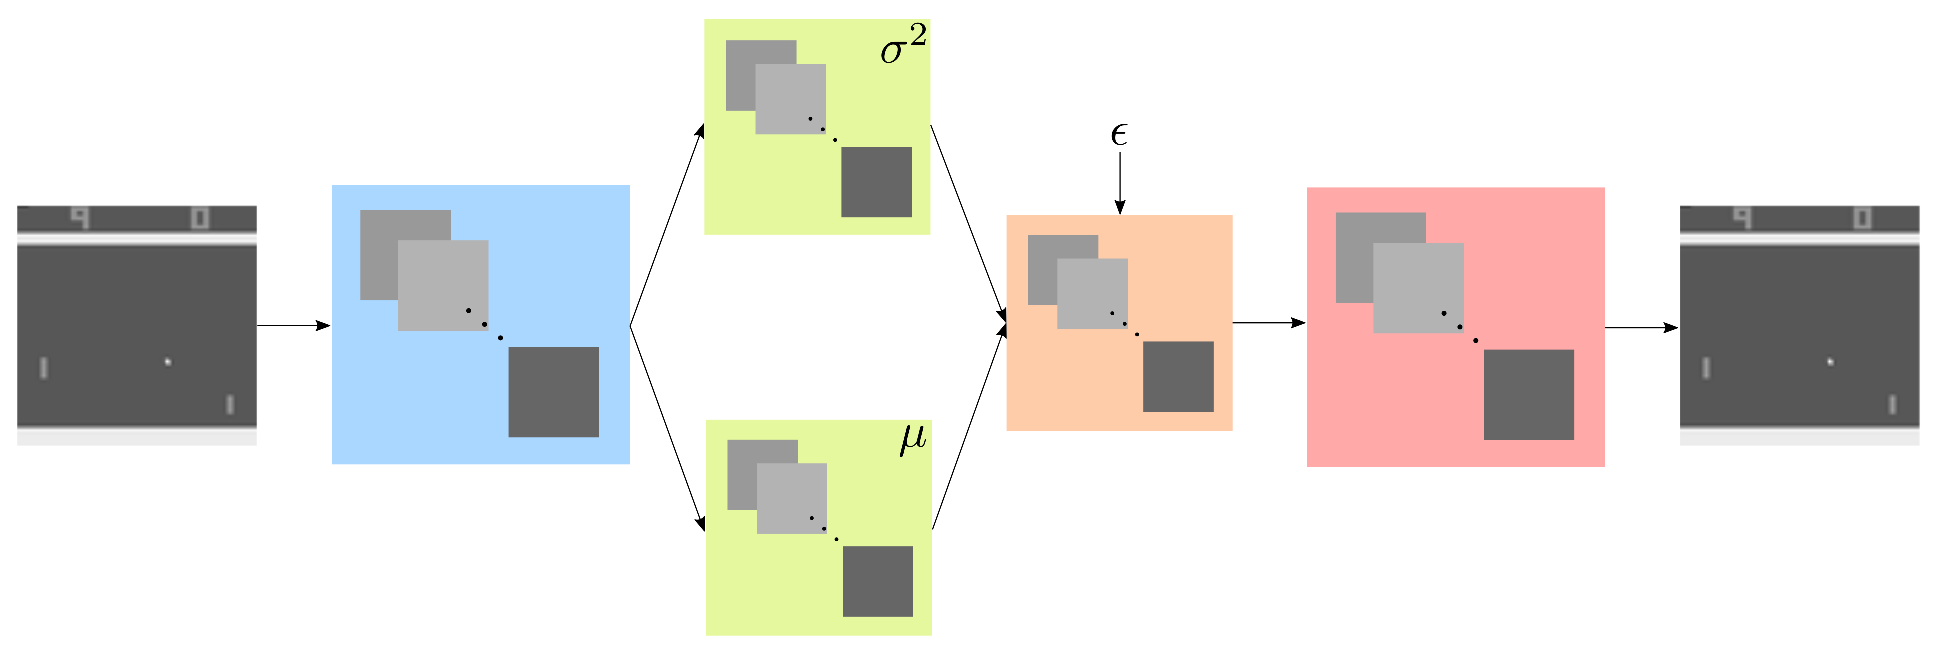
\includegraphics[scale=0.55]{methods/decoupling_indiscriminately_horizontal.eps}
\caption{Caption.}
\label{fig:decoupling_indiscriminately_horizontal}
\end{figure}

\begin{figure}[H]
\centering
\captionsetup{justification=centering}
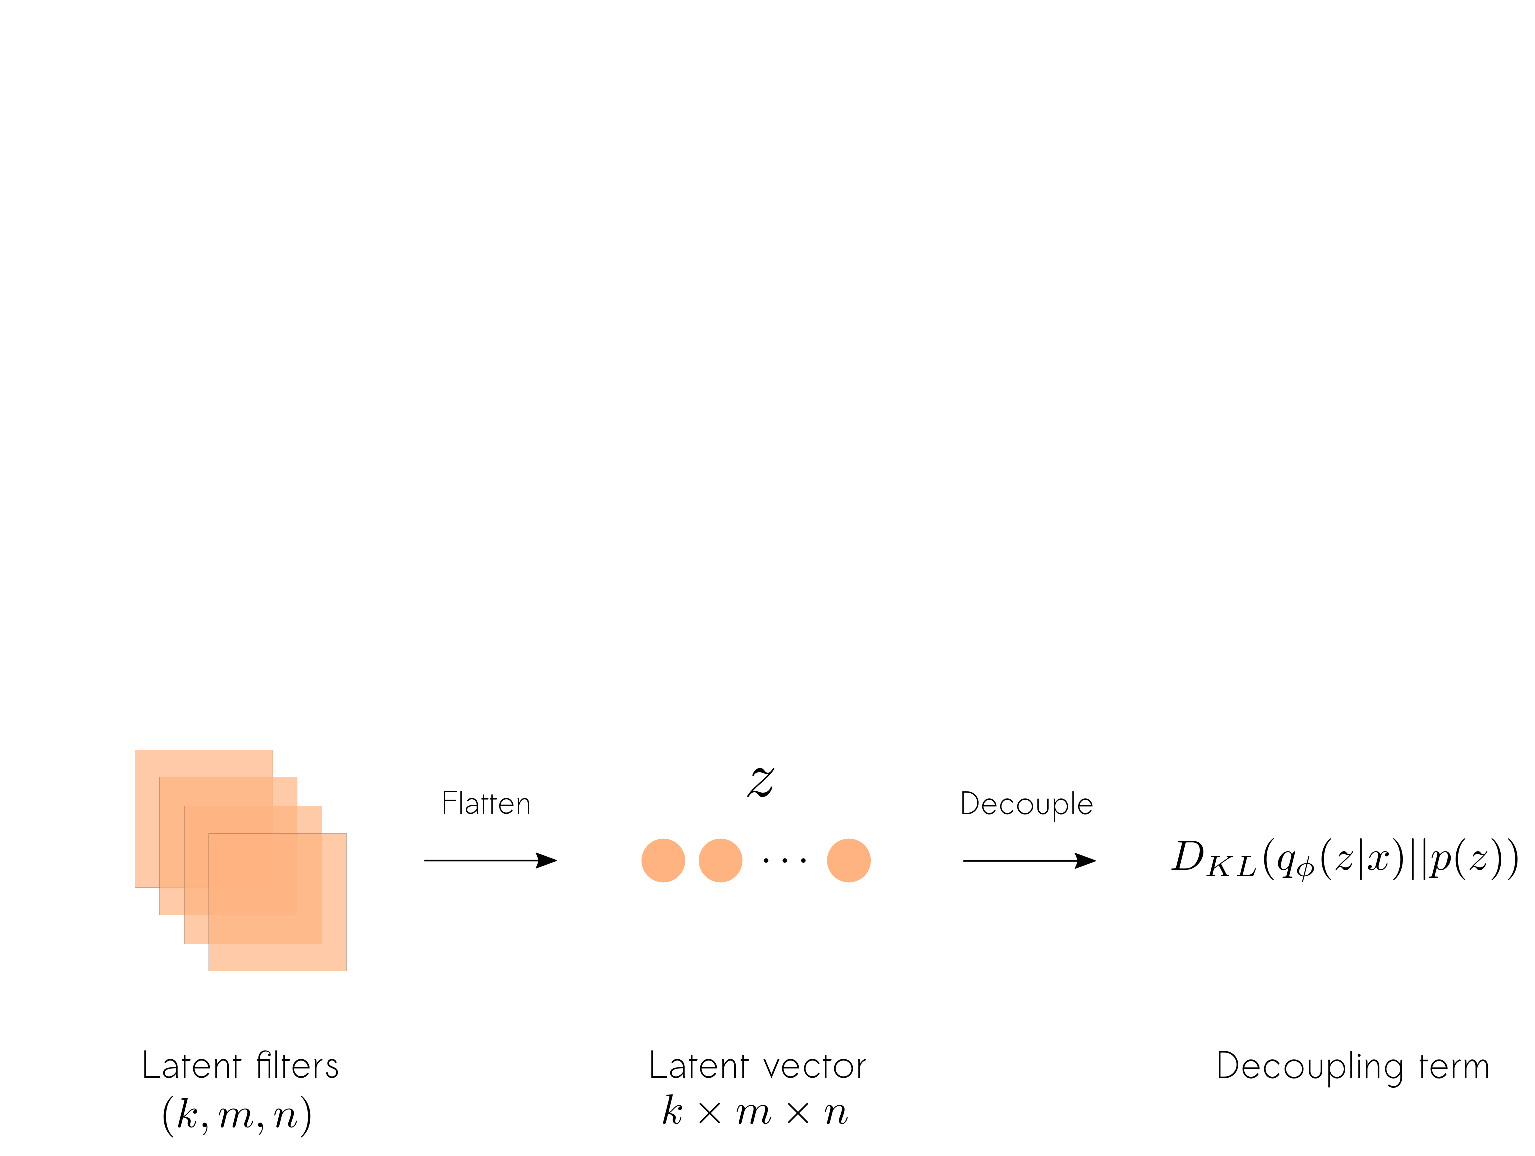
\includegraphics[scale=0.6]{methods/decoupling_indiscriminately_flattening_latent_space.eps}
\caption{Caption.}
\label{fig:decoupling_indiscriminately_flattening_latent_space}
\end{figure}

\subsection{Derivation}



%
%
%
%
%
\section{Disentangling Latent Filters Using Averages}
\lipsum[2]
\subsection{Architecture}
\begin{figure}[H]
\centering
\captionsetup{justification=centering}
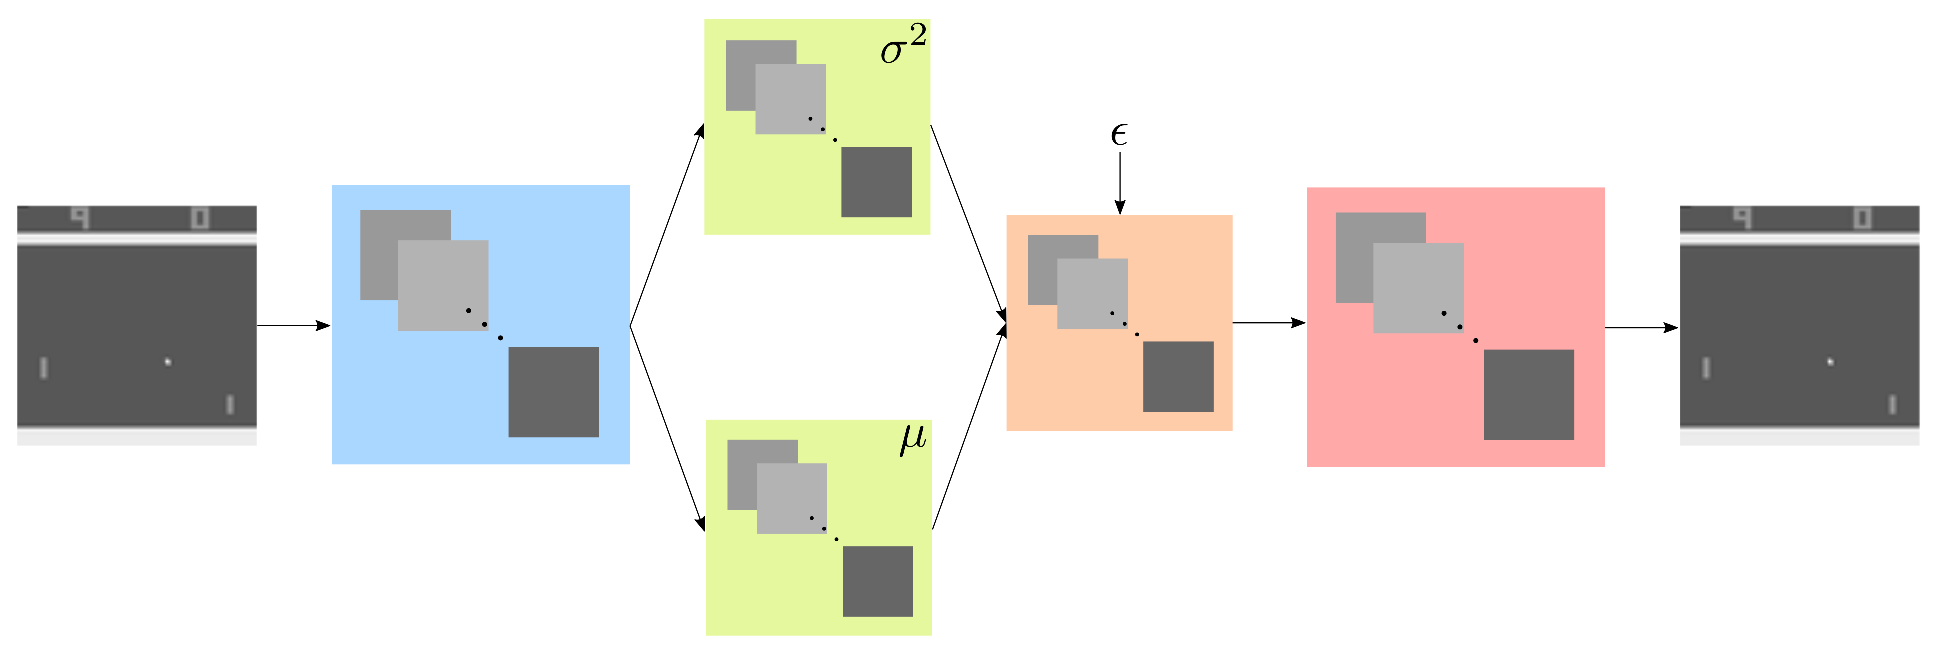
\includegraphics[scale=0.55]{methods/decoupling_indiscriminately_horizontal.eps}
\caption{Caption.}
\label{fig:decoupling_indiscriminately_horizontal}
\end{figure}

\begin{figure}[H]
\centering
\captionsetup{justification=centering}
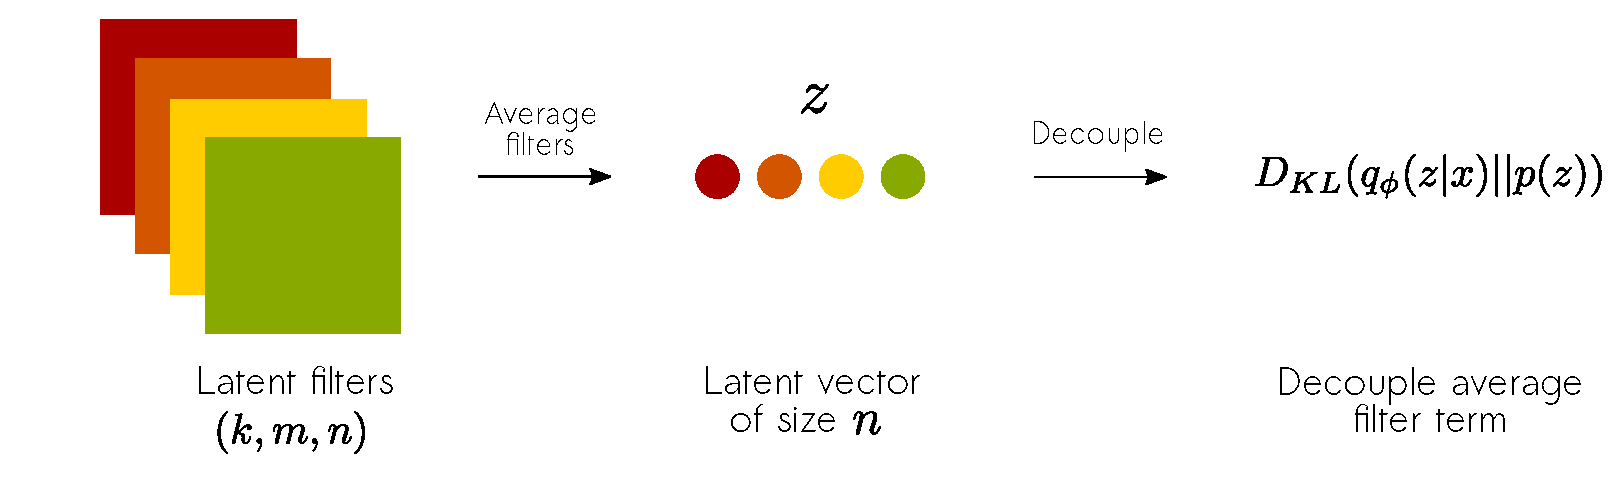
\includegraphics[scale=0.6]{methods/decoupling_averages_latent_space.eps}
\caption{Caption.}
\label{fig:decoupling_averages_latent_space}
\end{figure}

\subsection{Derivation}

%
%
%
%
%
\section{Decoupling Latent Filters Using Weighted-Averages}
\lipsum[2]
\subsection{Architecture}
\subsection{Derivation}

%
%
%
%
%
\section{Separating Colour Spaces}
\lipsum[2]
\subsection{Architecture}
\subsection{Derivation}

%
%
%
%
%
\section{Orthogonal Convolutions}
\lipsum[2]
\subsection{Architecture}
\begin{figure}[h!]
\centering
\captionsetup{justification=centering}
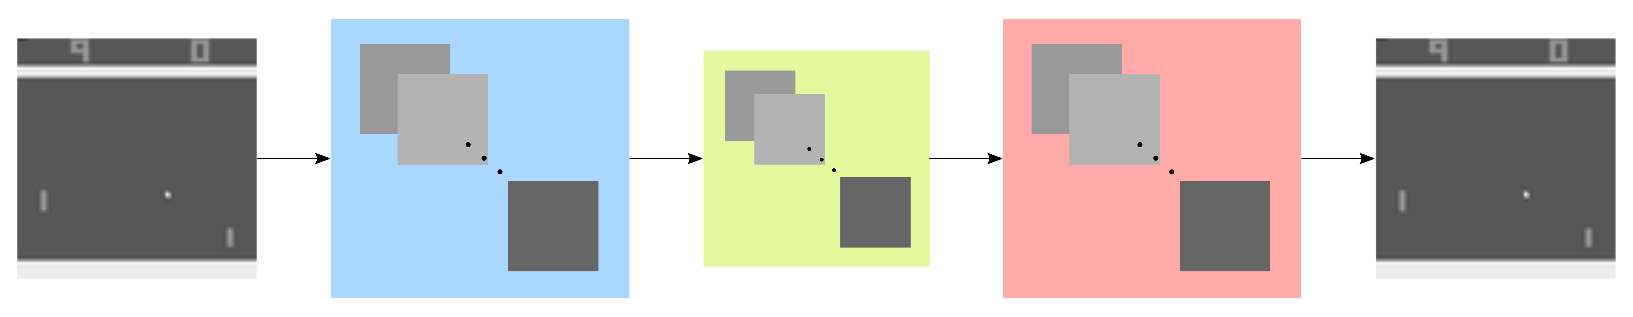
\includegraphics[scale=0.63]{methods/orthogonal_convolutions_archiecture.eps}
\caption{Caption.}
\label{fig:orthogonal_convolutions_archiecture}
\end{figure}

\subsection{Derivation}

%
%
%
%
%
\section{Winner Takes All}
\lipsum[2]
\subsection{Architecture}
\subsection{Derivation}
